\PassOptionsToPackage{table,svgnames}{xcolor} % Needed by dowecomment?
\PassOptionsToPackage{scaled=.8}{beramono} % Needed by showcode

% \documentclass[sigplan,screen]{acmart}
\documentclass[sigconf,review]{acmart}
%%
%% \BibTeX command to typeset BibTeX logo in the docs
\AtBeginDocument{%
  \providecommand\BibTeX{{%
    Bib\TeX}}}

%% Rights management information.  This information is sent to you
%% when you complete the rights form.  These commands have SAMPLE
%% values in them; it is your responsibility as an author to replace
%% the commands and values with those provided to you when you
%% complete the rights form.
\setcopyright{acmlicensed}
\copyrightyear{2018}
\acmYear{2018}
\acmDOI{XXXXXXX.XXXXXXX}
%% These commands are for a PROCEEDINGS abstract or paper.
% \acmConference[Conference acronym 'XX]{Make sure to enter the correct
%   conference title from your rights confirmation email}{June 03--05,
%   2018}{Woodstock, NY}
\acmConference[SPLC'25]{29th International Systems and Software Product Line Conference}{September 01--September 05, 2025}{A Coruña, Spain}
%%
%%  Uncomment \acmBooktitle if the title of the proceedings is different
%%  from ``Proceedings of ...''!
%%
%%\acmBooktitle{Woodstock '18: ACM Symposium on Neural Gaze Detection,
%%  June 03--05, 2018, Woodstock, NY}
\acmISBN{978-1-4503-XXXX-X/18/06}


%%
%% Submission ID.
%% Use this when submitting an article to a sponsored event. You'll
%% receive a unique submission ID from the organizers
%% of the event, and this ID should be used as the parameter to this command.
%%\acmSubmissionID{123-A56-BU3}

%%
%% For managing citations, it is recommended to use bibliography
%% files in BibTeX format.
%%
%% You can then either use BibTeX with the ACM-Reference-Format style,
%% or BibLaTeX with the acmnumeric or acmauthoryear sytles, that include
%% support for advanced citation of software artefact from the
%% biblatex-software package, also separately available on CTAN.
%%
%% Look at the sample-*-biblatex.tex files for templates showcasing
%% the biblatex styles.
%%

%%
%% The majority of ACM publications use numbered citations and
%% references.  The command \citestyle{authoryear} switches to the
%% "author year" style.
%%
%% If you are preparing content for an event
%% sponsored by ACM SIGGRAPH, you must use the "author year" style of
%% citations and references.
%% Uncommenting
%% the next command will enable that style.
%%\citestyle{acmauthoryear}


%%
%% end of the preamble, start of the body of the document source.

%%%%%%%%%%%%%%%%%%%%%%%%%%%%%%%%%%%%%%%%
\usepackage[greek,english]{babel}
\let\Bbbk\relax % Acmart load amssymb which defines \Bbbk
\usepackage{amssymb}
\usepackage{amsmath}
%%%%%%%%%%%%%%%%%%%%%%%%%%%%%%%%%%%%%%%%
%% Uncommenting the next command when the bios are needed
% \usepackage{wrapfig}
%%%%%%%%%%%%%%%%%%%%%%%%%%%%%%%%%%%%%%%%
% Use vector fonts, so it zooms properly in on-screen viewing software
% Don't change these lines unless you know what you are doing
\usepackage[T1]{fontenc}
\usepackage[utf8]{inputenc}
%%%%%%%%%%%%%%%%%%%%%%%%%%%%%%%%%%%%%%%%
\let\Bbbk\relax % Acmart load amssymb which defines \Bbbk
\usepackage{showcode}
%%%%%%%%%%%%%%%%%%%%%%%%%%%%%%%%%%%%%%%%
\usepackage[on]{dowecomment?}
\newcommand{\cwcomment}[1]{\usercomment{CW}{BloodRed}{#1}}
\newcommand{\bfcomment}[1]{\usercomment{BF}{Teal}{#1}}
%%%%%%%%%%%%%%%%%%%%%%%%%%%%%%%%%%%%%%%%
% Aliases
\newcommand{\tool}[1]{\textsc{#1}}
%%%%%%%%%%%%%%%%%%%%%%%%%%%%%%%%%%%%%%%%

\begin{document}

%%
%% The "title" command has an optional parameter,
%% allowing the author to define a "short title" to be used in page headers.
\title{The Name of the Title Is Hope}

%%
%% The "author" command and its associated commands are used to define
%% the authors and their affiliations.
%% Of note is the shared affiliation of the first two authors, and the
%% "authornote" and "authornotemark" commands
%% used to denote shared contribution to the research.
\author{Federico Bruzzone}
% \authornote{Both authors contributed equally to this research.}
\email{federico.bruzzone@unimi.it}
\orcid{0009-0004-6086-8810}
\affiliation{%
  \institution{Universit\`a degli Studi di Milano}
  \department{Computer Science Department}
  \city{Milan}
  \state{Italy}
  \country{Europe}}

\author{Walter Cazzola}
\authornote{Corresponding author.}
% \authornotemark[1]
\email{cazzola@di.unimi.it}
\orcid{0000-0002-4652-8113}
\affiliation{%
  \institution{Universit\`a degli Studi di Milano}
  \department{Computer Science Department}
  \city{Milan}
  \state{Italy}
  \country{Europe}}

%%
%% By default, the full list of authors will be used in the page
%% headers. Often, this list is too long, and will overlap
%% other information printed in the page headers. This command allows
%% the author to define a more concise list
%% of authors' names for this purpose.
\renewcommand{\shortauthors}{Bruzzone and Cazzola}

%%
%% The abstract is a short summary of the work to be presented in the
%% article.
\begin{abstract}
  A clear and well-documented \LaTeX\ document is presented as an
  article formatted for publication by ACM in a conference proceedings
  or journal publication. Based on the ``acmart'' document class, this
  article presents and explains many of the common variations, as well
  as many of the formatting elements an author may use in the
  preparation of the documentation of their work.
\end{abstract}

%%
%% The code below is generated by the tool at http://dl.acm.org/ccs.cfm.
%%
\begin{CCSXML}
  <ccs2012>
     <concept>
         <concept_id>10003752.10010124.10010138.10010143</concept_id>
         <concept_desc>Theory of computation~Program analysis</concept_desc>
         <concept_significance>500</concept_significance>
         </concept>
     <concept>
         <concept_id>10011007.10011006.10011041</concept_id>
         <concept_desc>Software and its engineering~Compilers</concept_desc>
         <concept_significance>300</concept_significance>
         </concept>
   </ccs2012>
\end{CCSXML}

\ccsdesc[500]{Theory of computation~Program analysis}
\ccsdesc[300]{Software and its engineering~Compilers}

%%
%% Keywords. The author(s) should pick words that accurately describe
%% the work being presented. Separate the keywords with commas.
\keywords{Do, Not, Us, This, Code, Put, the, Correct, Terms, for,
  Your, Paper}
%% A "teaser" image appears between the author and affiliation
%% information and the body of the document, and typically spans the
%% page.
% \begin{teaserfigure}
  % 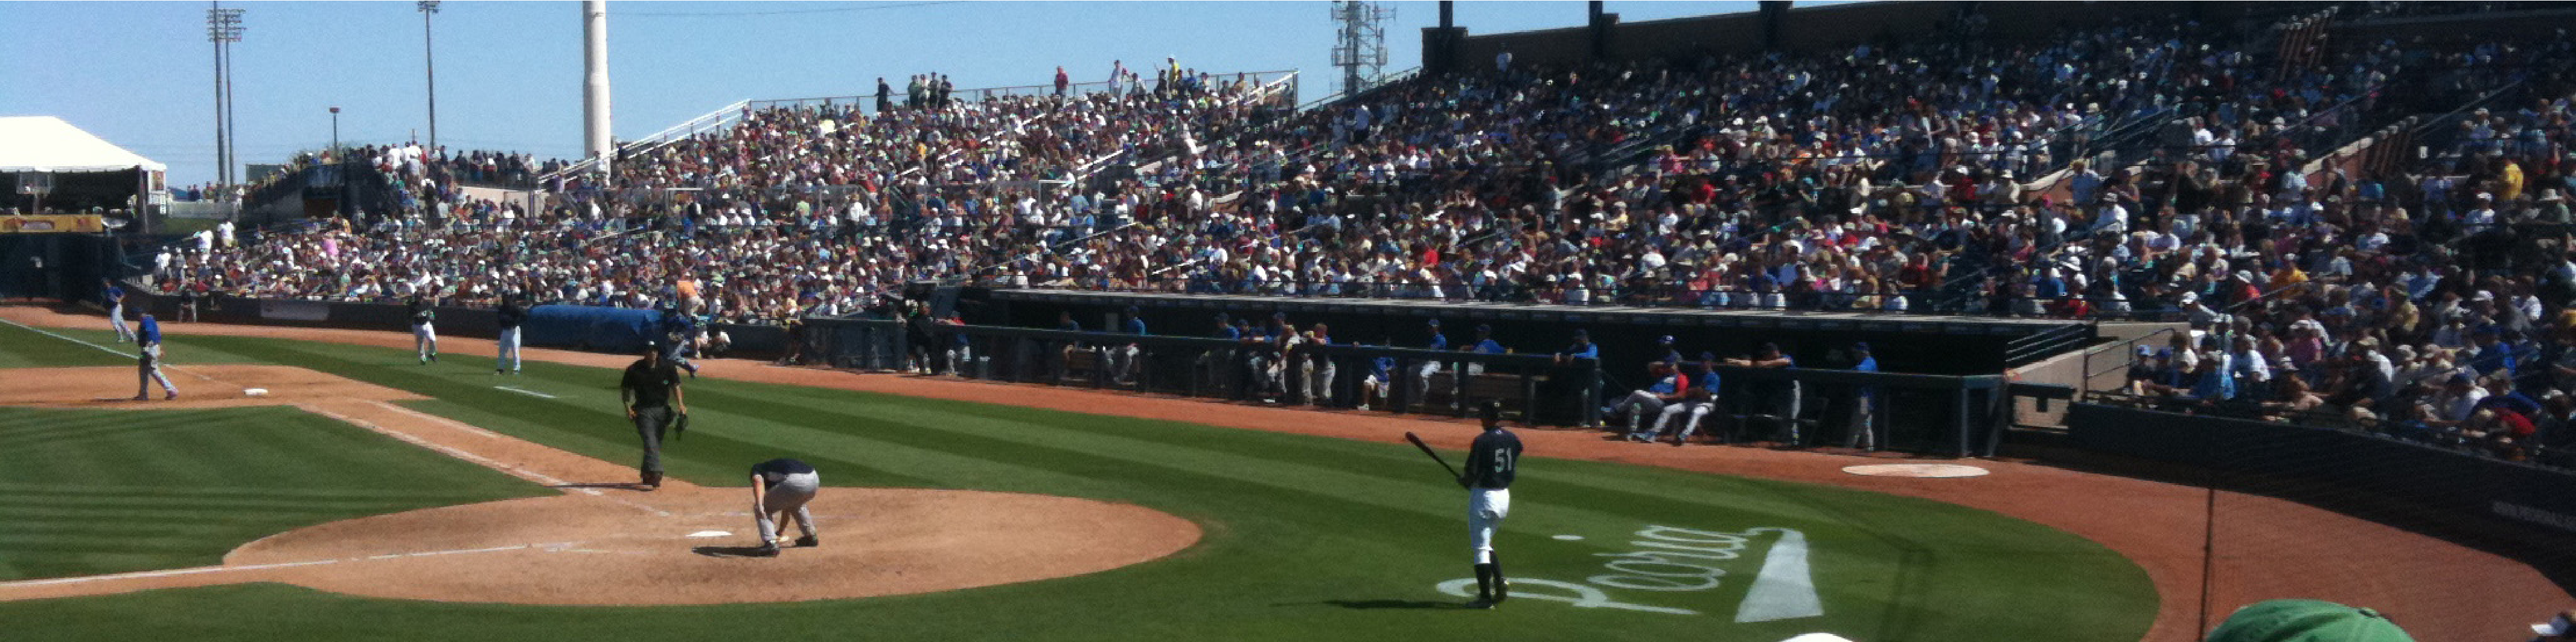
\includegraphics[width=\textwidth]{sampleteaser}
  % \caption{Seattle Mariners at Spring Training, 2010.}
  % \Description{Enjoying the baseball game from the third-base
  % seats. Ichiro Suzuki preparing to bat.}
  % \label{fig:teaser}
% \end{teaserfigure}

\received{20 February 2007}
\received[revised]{12 March 2009}
\received[accepted]{5 June 2009}

%%
%% This command processes the author and affiliation and title
%% information and builds the first part of the formatted document.
\maketitle

\section{Introduction}
\section{Background}\label{sec:bg}

In this section, we introduce some preliminary concepts that are necessary to understand the rest of the paper. 
% Rust
We start by introducing the Rust programming language and its ownership system.
% SPL and SPL testing
Then, we introduce the concept of software product lines (SPLs) and the importance of testing SPLs.
% Centrality measures
Finally, we provide an overview of centrality measures in graph theory, which are necessary to understand the approach we propose in this paper.

\subsection{The Rust Programming Language}\label{subsec:bg:rust}

Rust is a systems programming language that focuses on safety, speed, and concurrency. It is designed to be memory-safe without using garbage collection. 
This implies that pure Rust programs are free of null pointer dereferences, double frees as well as data races.
The \emph{linear logic}~\cite{Girard87, Girard95} and \emph{linear types}~\cite{Wadler90, Odersky92}---which force the use of resources exactly once---inspired the \emph{ownership} system.
Rust incorporates it into its type system as relaxed form of pure linear types to ensure type soundness.
The ownership system ensures that there is only one \emph{owner} (the variable binding) for each piece of memory (a value) at any given time, and when the owner goes out of scope or is otherwise deallocated, the memory is deallocated as well. By leveraging the latter property, Rust supports user-defined destructors, enabling \emph{resource acquisition is initialization} (RAII) pattern proposed by Stroustrup~\cite{Stroustrup94}.
The lifetime of the owned value is determined by the scope in which the owner takes ownership.
An owner can \emph{move} (transfer) the ownership of the value to a new owner or \emph{borrow} the value to another part of the program.
By \emph{moving} the ownership, the previous owner can no longer access the value.
On the other hand, Rust support \emph{references} that allow the owner to \emph{borrow} the value avoiding the its invalidation.
Two kind of \emph{borrows} are supported: \emph{immutable} and \emph{mutable}.
Multiple \emph{immutable borrow} can coexist, but only one \emph{mutable borrow} can exist at a time. 
These restrictions allow Rust to guarantee memory safety. Furthermore, the lifetime of a reference can not outlive (exceed) the lifetime of the owner, which ensures no dangling pointers.
The Rust compiler enforces all these rules at compile time also by performing \emph{borrow checking}, preserving the runtime performance of the compiled code.
Despite the notable progress in the field of safe systems programming, Rust allows \inlinerust{unsafe} blocks to perform low-level operations that are not safe, such as dereferencing raw pointers.
In Rust, the \inlinerust{unsafe} keyword signifies that the responsibility for preventing undefined behavior shifts from the compiler to the programmer. This ensures that undefined behavior cannot occur in safe Rust code, as the compiler enforces strict safety guarantees in all safe contexts.

\subsection{Product Families}\label{subsec:bg:spl}

In product families the similarities and differences are characterized by a set of features \(F = \{f_1, f_2, \ldots, f_m\}\) where each feature \(f_i \subseteq A\).
A feature is a unit that provides a piece of functionality that satisfies a requirement or represents a design decision and fixed \(i\) and \(j\) such that \(i \neq j \centernot\implies f_i \cap f_j = \emptyset\).
A product line, or rather a family of products, is a set of products \(P = \{p_1, p_2, \ldots, p_k\}\) where each product \(p_i \subseteq F\) is a set of features and for fixed \(i\) and \(j\) such that \(i \neq j\), it does not necessarily follow that \(p_i \cap p_j = \emptyset\).
A key task in SPL engineering is feature modeling, which involves creating and maintaining a \emph{feature model}. The concept of feature model was first introduced by~\citet{Kang90} in the FODA method and serves to represent the variability of a system through its features and their interdependencies. In SPLs, the feature model formalism is essential for configuring software products by defining valid feature sets, known as \emph{configurations}. 
A configuration \(c:F\rightarrow \{0, 1\}\) is a characteristic function over \(F\) that maps each feature to a boolean value. 
A feature $f$ is considered \emph{active} if it belongs to a configuration \(c\) such that \(c(f)=1\), otherwise it is \emph{inactive}.
The structure of a feature model implicitly captures feature dependencies by specifying mandatory, optional, alternative, and grouped features. These dependencies are often represented as parent-child relationships, where a feature can only be \emph{active} if all its parent features are also \emph{active}. 
A configuration \(c\) is deemed \emph{valid} if and only if \(\forall f_i\in F\mid c(f_i)=1\implies\exists p\in P\mid f_i\in p\).
Given a product \(p_i \in P\) we say that all products \(p_j \in P\) such that \(p_j \neq p_i\) are variants of \(p_i\) denoted as \(v_j\).
It is worth noting that a family of products \(P\) can theoretically contain up to \(2^{|F|}\) variants, as described by~\citet{Krueger06}. This exponential growth in potential configurations has paved the way for the development of techniques to manage and test SPLs effectively~\cite{Pohl06}.
Numerous approaches, recently analyzed by~\citet{Agh24}, have been proposed to address the challenges of testing SPLs, including product sampling~\cite{Patel13, AlHajjaji19, Lee19} and combinatorial testing~\cite{Oster10, Lochau12}.

\subsection{Centrality Measures}\label{subsec:bg:centrality}



\section{Related Work}\label{sec:related-work}

\bfcomment{Nella sezione 4.4 di \cite{Agh24}}
\bfcomment{Guardare le precedenti literature review}

%%
%% The acknowledgments section is defined using the "acks" environment
%% (and NOT an unnumbered section). This ensures the proper
%% identification of the section in the article metadata, and the
%% consistent spelling of the heading.
\begin{acks}
\bfcomment{TODO}
\end{acks}

%%
%% The next two lines define the bibliography style to be used, and
%% the bibliography file.
\bibliographystyle{ACM-Reference-Format}
% \bibliography{sample-base}
\bibliography{local,strings,metrics,programming,software_engineering,software_architecture,dsl,pl,splc,oolanguages,my_work,grammars,security,roles,learning,cop,testing,dsu,distributed_systems,reflection,aosd,pattern,logic}

% \input sects/bios

%%
%% If your work has an appendix, this is the place to put it.
\appendix

\section{Appendix 1}

\subsection{Part One}

\bfcomment{TODO}

\subsection{Part Two}

\bfcomment{TODO}

\section{Appendix 2}

\section{Part One}


\end{document}
\endinput
